
%<><><><><><><><><><><><><><><><><><><><><><><><><><><><><><><><><><><><><><><><><><><><><>
 % Backgrounds
 %<><><><><><><><><><><><><><><><><><><><><><><><><><><><><><><><><><><><><><><><><><><><><>
\section{Backgrounds}

\begin{figure}[tbp]
\begin{center}
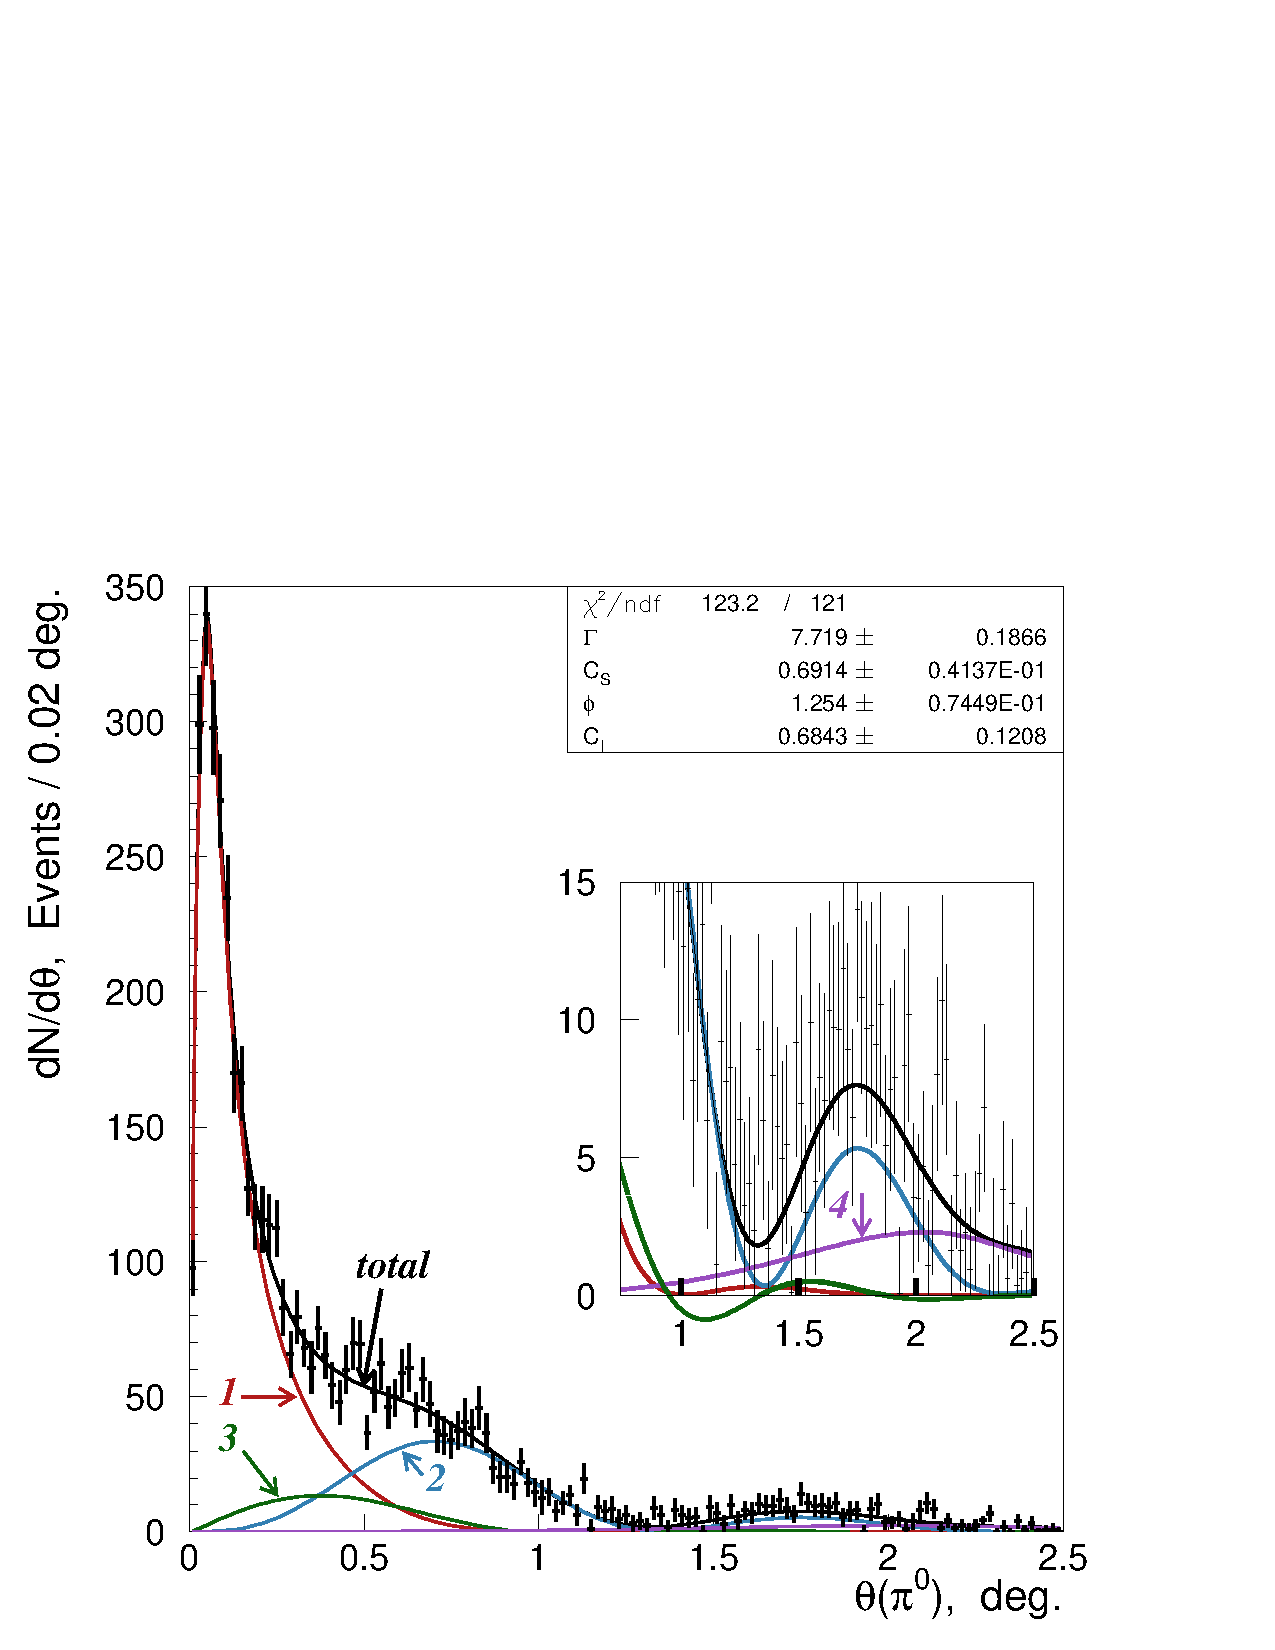
\includegraphics[width=8cm,angle=0,trim={1.5cm 0.5cm 3.5cm 9.5cm},clip]{figures/dndt_pb_partial.pdf}
\end{center}
\caption{Exclusive $\pi^0$ production yield at forward angle on lead target
observed in the PrimEx experiment \cite{Larin:2010kq}. Curves show production mechanisms input:
1 -- Primakoff, 2 -- strong coherent, 3 -- interference of first two mechanisms, 4 -- strong incoherent}
\label{fig:leaddndt}
\end{figure}




% \begin{landscape}
\begin{table}[t]
\caption{Comparison of backgrounds for the single $\pi^0$ channel and the present study for 
determination of the signal in the $\pi^0\pi^0$ channel. The relative backgrounds for this experiment
are expected to be smaller than those for the single $\pi^0$ channel.
\label{tab:Primex_sigmas}
}
\begin{center}
\begin{tabular}{|l|c|c|}
\hline
\hline 
 Integrated Fraction & $\gamma\,Pb\to \pi^0\, Pb$  & $\gamma\,Pb\to \pi^0\pi^0\, Pb$ \\  
  ($\theta <$ 1.5 degrees)                    &       & (This study) \\  \hline
  Primakoff signal  &   1.0   & 1.0   \\ \hline 
  Nuclear Coherent (NC)  & 0.39  &   0.35   \\ \hline 
  Interference  & 0.12  &  0.17   \\ \hline 
  $\gamma p \rightarrow \eta p$, BR($\eta \rightarrow 3\pi^0$)  &   -- & 0.37   \\ \hline 
  Incoherent (IC)  &   0.02  & 0.06  \\
  \hline   
  \hline
\end{tabular}
\end{center}
\end{table}





\begin{figure}[tbp]
\begin{center}
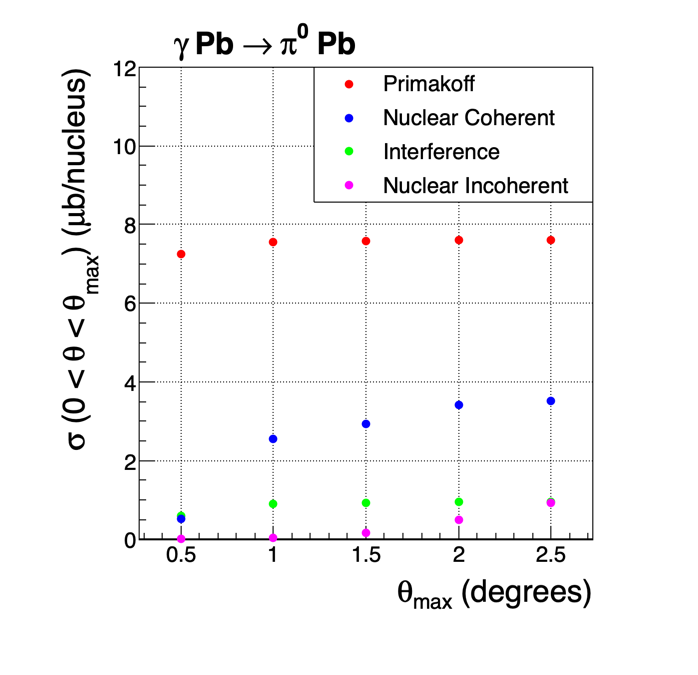
\includegraphics[width=7cm,angle=0]{figures/Primex_sigmas_c1.png}
\end{center}
\caption{Integrated angular distribution for different components to $\pi^0$ production in $\gamma\,Pb\rightarrow\pi^0\,Pb$ as a function of the upper limit of integration.}
\label{fig:Primex_sigmas_c1}
\end{figure}


We first classify the various backgrounds and then describe them in more detail one at a time. There are two-pion production data on nuclei below 2~GeV \cite{schadm2005double} in a kinematic regime that is dominated by nucleon resonances. However, at our energy of 6 GeV, 
the exclusive production of two pions at threshold is very poorly known experimentally, and therefore there are large uncertainties in both the magnitude and the expected distributions of the backgrounds.  The major background comes from the $f_0(500)$ $0^{+}$ meson (also referred to as $\sigma$-meson in the literature) that decays to two pions. The production mechanism is expected to be very similar to single $\pi^0$ $0^{-}$ production, since the final states are similar except for parity. Therefore, we assume the {\em relative} background contributions in the single $\pi^0$ reaction will be similar in our experiment. The single-pion production distribution on a lead target measured by PrimEx \cite{Larin:2018} is shown in Fig\,\ref{fig:leaddndt}. The relative contributions for $\pi^0$ production are plotted in Fig.\,\ref{fig:Primex_sigmas_c1} as a function of angle, highlighting the fact that the Primakoff process is very forward peaked. The integrated fractions are also tabulated for $\theta < 1.5$ degrees in Table\,\ref{tab:Primex_sigmas} and compared to fractions used in this study.
Production inside the nucleus will tend to reduce hadronic backgrounds in the 2$\pi$ case due to absorption, but we take a conservative approach that absorption does not change the general picture substantially. 

 \begin{figure}[tbh]
\begin{center}
%\includegraphics[height=5cm,viewport=250 180 0 360,clip=true]{CPP_production3}
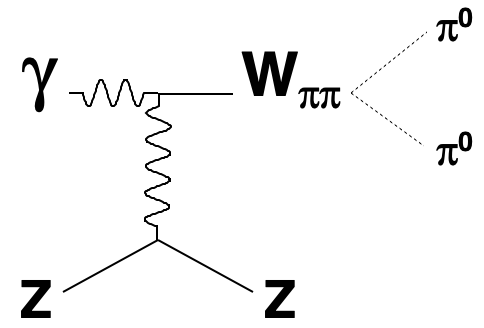
\includegraphics[height=3cm,clip=true]{figures/Diagram_Primakoff.png} \hspace{1cm}
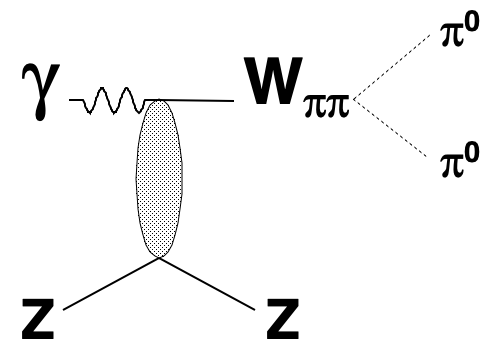
\includegraphics[height=3cm,clip=true]{figures/Diagram_hadronic.png}
\caption{Sketch of coherent two-pion production. Left) Signal: Primakoff mechanism, Right) Backgrounds: Other production mechanisms.
\label{fig:Diagram}}
\end{center}
\end{figure}

We have the following categories of backgrounds:
\begin{itemize}
\item Nuclear coherent production: In this case, the target remains intact. Generically, one may classify the two-pion production
according to the sketches in Fig.\,\ref{fig:Diagram}. The left-hand diagram represents the exchange of a virtual photon with the nucleus, i.e. the Primakoff
mechanism. This mechanism is very long range, approximately 100 fm, and is affected minimally by the effects of shadowing or absorption.  This is the signal for the
experiment and our goal is to determine its cross section.
The right-hand diagram represents the exchange of a strongly interacting particle (or propagator) and effectively results in the production of pions at the
surface of the nucleus. We note that for the $\pi^0\pi^0$ production, pion exchange is not allowed due to charge conjugation conservation, while 
in the $\pi^+\pi^-$ case, single pion exchange is related to the axial anomaly ($\gamma \pi^0 \rightarrow \pi^+ \pi^-$).  When the interaction leaves the
nuclear target intact, the reaction is referred to as ``nuclear coherent'' and this is one of our most serious backgrounds. 
\item Incoherent production:  When the interaction produces two pions in the quasi-elastic scattering off a single
nucleon, the scattered target usually fragments into particles that range out in the target and are unobserved experimentally. This reaction occurs at larger $-t$ and is in general
kinematically distinct from the signal. The $\pi^0\pi^0$ momentum relative to the photon polarization plane does differentiate between the Primakoff and incoherent production.
\item Any reaction that may be confused with the signal within the experimental resolution or limited acceptance:
 An example of this type of reaction is Primakoff production of $\eta$ mesons, where the $\eta\rightarrow \pi^0 \pi^0 \pi^0$  is
mis-reconstructed as a two-pion final state. 
\end{itemize}

We note that two important backgrounds for the charged-pion polarizability experiment do not contribute in this experiment:
First, coherent $\rho^0$ photo-production is absent in this
experiment because the $\rho^0$ decay into the $\pi^0\pi^0$ channel is prohibited by I-spin conservation.  Second, $\mu^+\mu^-$ production is also not a factor in the neutral pion case.

\subsection{Nuclear coherent background \label{sec:NCback}}
   
 The largest coherent backgrounds are  
from the photoproduction of the $f_0(500)(J^{PC}=0^{++})$ and the $f_0(980)$.  The width of the
$f_0(980)$ is fairly narrow and does not contribute directly to the strength near threshold.
The $f_0(500)$ width is much
broader, from threshold to 800 MeV, with significant overlap in the
invariant mass region of interest.  Since the $f_0(500)$ is a scalar
particle with the same spin-parity as the $\gamma \gamma \rightarrow
\pi^0\pi^0$ final state near threshold, the azimuthal distribution of the $\pi^0\pi^0$ momentum relative to the
photon polarization plane does not differentiate between coherent
$f_0(500)$ production and the Primakoff reaction.  
This is similar to the PrimEx-$\pi^0$ experiment, where the dominant background was
nuclear coherent $\pi^0$ photo-production.  The approach used in the
PrimEx analysis was to measure the $\pi^0$ angular distribution,
effectively the $t$-distribution, then use theoretical calculations of
the angular distributions to separate out contributions from Primakoff
and nuclear coherent. The analysis of the $\pi^0\pi^0$ (NPP) reaction
will approximately mirror what was done for the PrimEx-$\pi^0$
analysis.  

We parameterize the $f_{0}(500)$ meson as detailed in Appendix\,\ref{sec:NCsigma} and assume that the production amplitude can be factorized as
\begin{eqnarray}
\mathcal{A} & = & \mathcal{A}_t(t) \, \mathcal{A}_W(m_{\pi\pi}) \, \mathcal{A}_\tau(\Phi, \phi, \theta),
\end{eqnarray}
where the last factor represents the angular distribution that results in a 
dependence on the di-pion azimuthal angle, $\phi_{\pi\pi}$, of the form $\mathcal{A}_\tau \propto (1 + \mathcal{P} \cos{2\phi_{\pi\pi}}$). 
The mass dependence is given by the S-wave phase shifts that dominate the mass region below 0.8 GeV. We use the approximate description given in 
Appendix\,\ref{sec:ParmSwave}.\footnote{More detailed studies may require including contributions from the D-wave and S-wave, I=2, amplitudes.} 

 \begin{figure}[tbh]
\begin{center}
%\includegraphics[height=5cm,viewport=250 180 0 360,clip=true]{CPP_production3}
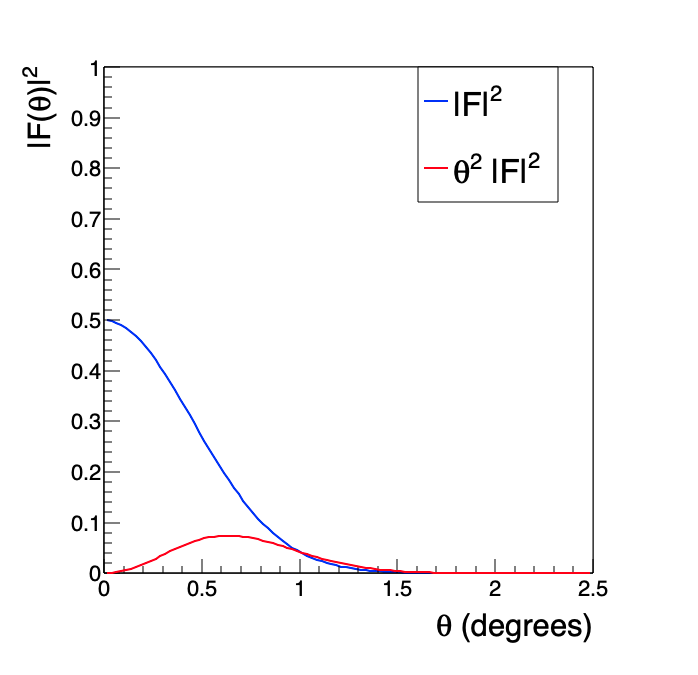
\includegraphics[height=5cm,clip=true]{figures/fit_Primakoff_sigma_c1.png}
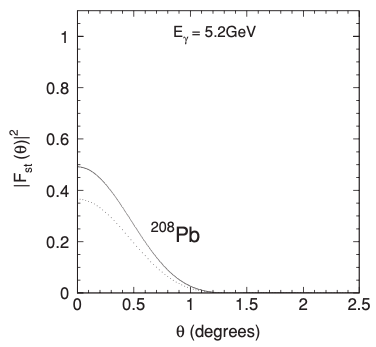
\includegraphics[height=5cm,clip=true]{figures/PRC80_2009_Fig6.png}
\caption{ Left) Approximation to strong form factor for lead, Right) Figure 6 from Ref.\,\cite{Gevorkyan:2009ge} showing the calculated strong form factor for single $\pi^0$ production off a lead target.
\label{fig:strongFF}}
\end{center}
\end{figure}

We assume the $-t$ dependence of the $f_0(500)$ has a similar functional form as single $\pi^0$ production, namely $\mathcal{A}_t(t) \propto \sin{\theta_{\pi\pi}} \times F_{st}(t)$.  The $\sin{\theta_{\pi\pi}}$ 
comes from the spin-flip required at forward angles to produce a $0^+$ system off a spin-zero target. The factor $F_{st}(t)$ is the strong form factor for the target, which is approximated to
match calculations for the single $\pi^0$ production (Fig.\,6 from Ref.\cite{Gevorkyan:2009ge}). Our Gaussian approximation to the form factor is shown in Fig.\,\ref{fig:strongFF} along side the calculation for single 
$\pi^0$ production. Efforts are underway to calculate the strong form factor for this reaction.\footnote{S. Gevorkyan, private communication.}
The PrimEx data showed that the nuclear coherent process is highly
suppressed for heavy nuclei, as shown in Fig.\ref{fig:leaddndt}.  The reason for this suppression is
$\pi^0$ absorption in the nuclear interior, making the coherent
production primarily a surface effect.  For NPP it is expected that suppression of the nuclear  
coherent process will be approximately twice stronger than that seen in PrimEx because two pions
are produced in NPP as compared to a single $\pi^0$ in PrimEx. 

 \begin{figure}[tbp]
\begin{center}
%\includegraphics[height=5cm,viewport=250 180 0 360,clip=true]{CPP_production3}
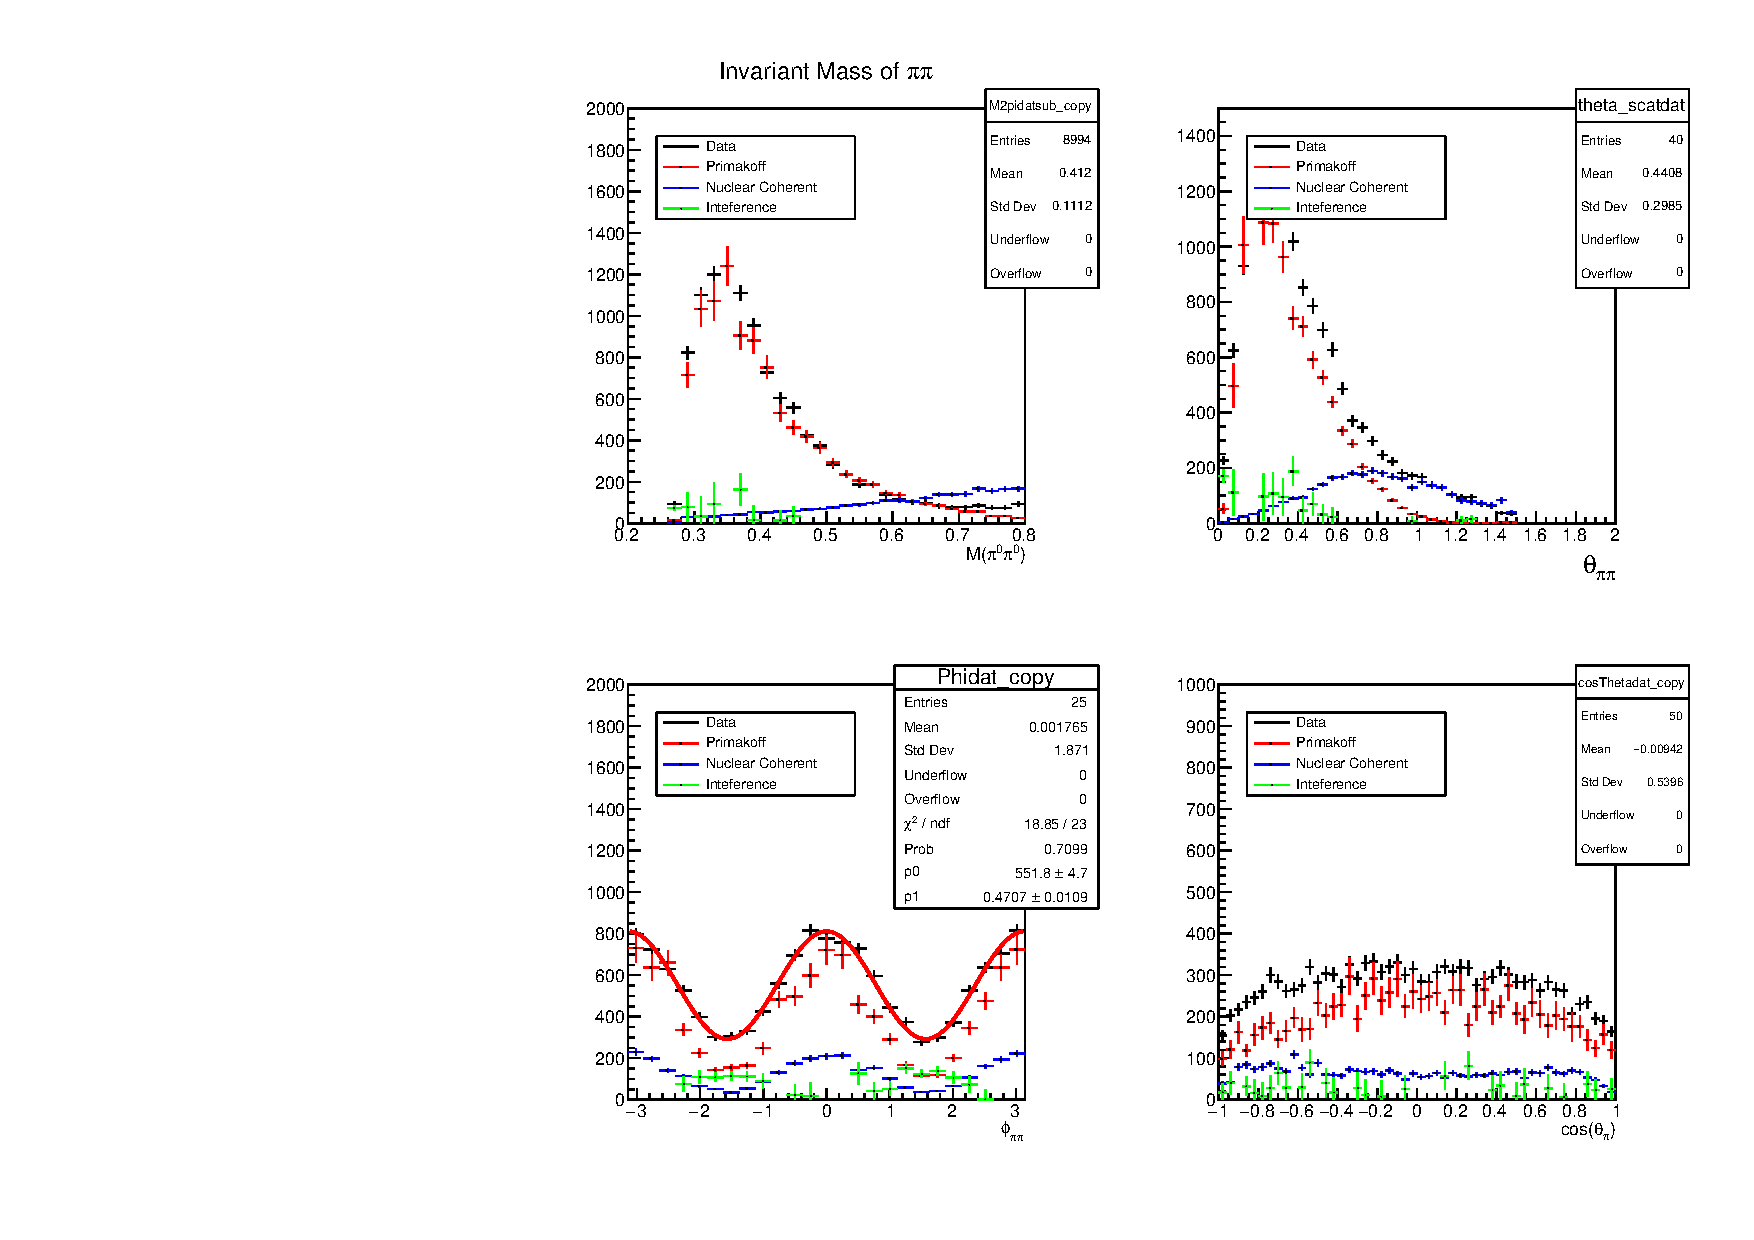
\includegraphics[height=15cm,clip=true]{figures/twopi_primakoff_DSelect_test_File_100000_decomposition_PrimNC.pdf}
\caption{Kinematic distributions for the Primakoff signal and nuclear coherent background only are shown for reference. The MC data (black) are fitted to the sum of the signal and NC background including the interference between amplitudes. 
Top left) 2$\pi$ mass, Top right) 2$\pi$ scattering angle, Bottom left) 2$\pi$ azimuthal angle, 
Bottom right) Polar angle of one pion in the $2\pi$ center-of-mass.
\label{fig:decomposition_PrimNC}}
\end{center} 
\end{figure}

Figure\,\ref{fig:decomposition_PrimNC} shows distributions of interest for a sample of $\pi^0\pi^0$ Primakoff and
nuclear coherent background events simulated in approximate proportion observed in single pion production. The strong phase between the two production mechanisms is set to
75 degrees for this simulation, where an angle of zero produces maximum interference. This angle must be determined experimentally. 
The 2$\pi$ mass and the 2$\pi$ scattering angle distributions are shown in the top two panels. The Primakoff signal peaks at the 2$\pi$-mass threshold and at about 0.2 degrees, whereas the nuclear coherent signal rises linearly from 2$\pi$ threshold, as expected for $f_0(500)$ production, and peaks at an angle of about 0.75 degrees. The azimuthal angular distribution is the same for both signal and background and has no discriminating power. The angular distributions of the pions in
the center of mass of the $2\pi$ system are all uniform, and as such do not help in distinguishing the signal from the nuclear coherent.  

\begin{figure}[tbp]
\begin{center}
%\includegraphics[height=5cm,viewport=250 180 0 360,clip=true]{CPP_production3}
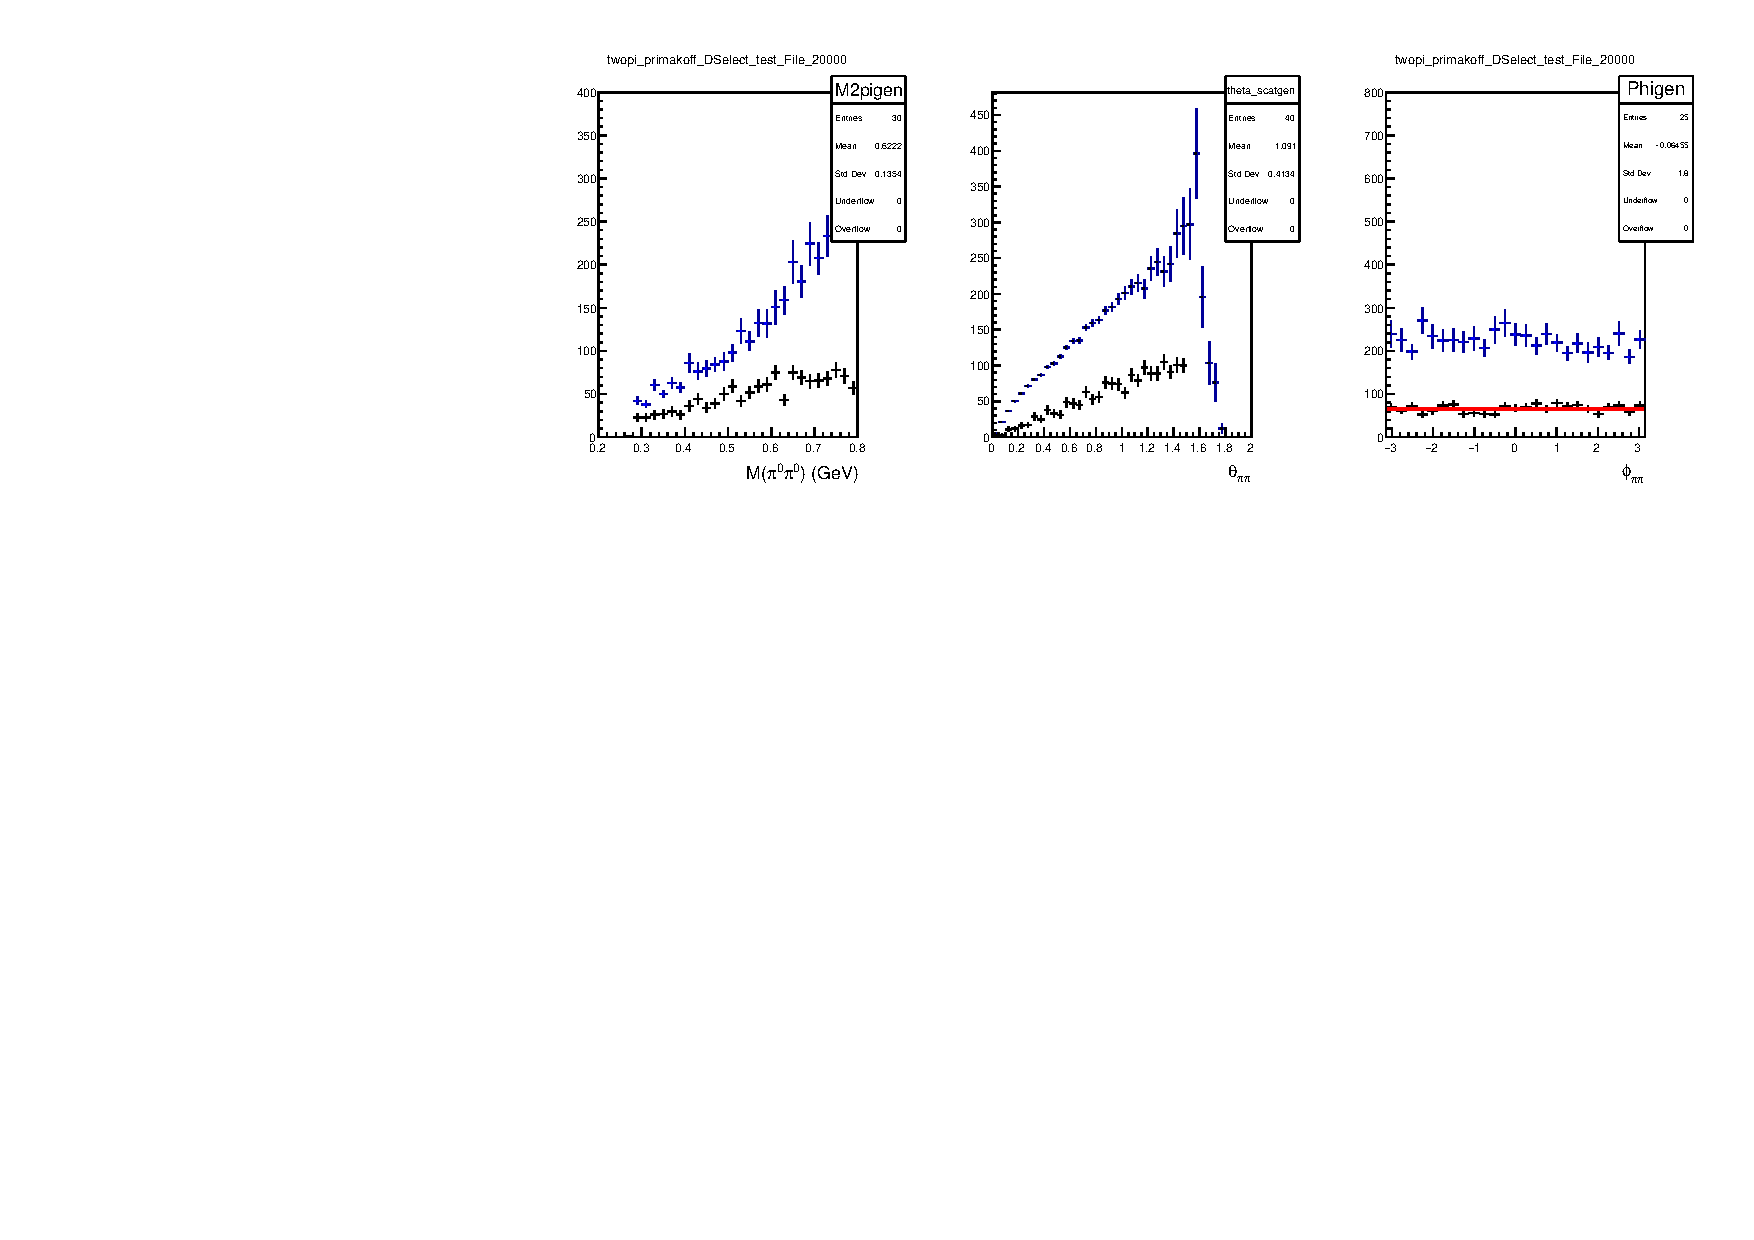
\includegraphics[width=16cm,clip=true]{figures/twopi_primakoff_DSelect_test_File_20000_IC.pdf}
\caption{Distributions for the incoherent production off free nucleons. The blue crosses represent the generated distributions and the black crosses represent the kinematically fit accepted distributions.
Left) 2$\pi$ mass. Center) 2$\pi$ scattering angle. The drop of the generated distribution at 1.5 degrees is due to an analysis cut. Right) 2$\pi$ azimuthal angle.
\label{fig:IC}}
\end{center} 
\end{figure}

\subsection{Incoherent two-pion production}
In addition to the coherent production of two pions off the nucleus, two pions may also be produced via the elementary reaction $\gamma N\to \pi^0 \pi^0 N$, breaking up the nucleus in the process. We model the incoherent background with a mass distribution given by the $f_0(500)$, but with an exponential $t$ dependence given by $e^{Bt}$, with $B=3.6$ GeV$^{-2}$. The slope is taken from Ref.\cite{Battaglieri:2009aa} and has very large uncertainties. However, as long as the slope is small compared to Primakoff production, which has an effective slope of $B\sim560$ GeV$^{-2}$, it does not change the picture. The mass and angular dependencies are shown in Fig.\,\ref{fig:IC}. The strength is small at threshold and at small angles, where Primakoff is strongest. The azimuthal angle is flat, so the photon polarization can also discriminate against this background. 

The cross section for this reaction on free protons is relatively large, about 140 nb/nucleon  for $0.3 < M_{\pi\pi} < 0.8$ GeV.\footnote{The cross section is estimated from the S-wave production of the $f_0(500)$ meson extrapolated to small $-t$ from data archived in the {\em hepdata.net} database and reported in Ref.\,\cite{Battaglieri:2009aa}. See Appendix\,\ref{sec:NCsigma} for more information. A factor of one half is applied to the measured cross section for $\pi^+\pi^-$.} However, this process is strongly suppressed in nuclei by Pauli blocking and by pion absorption. The Pauli suppression is proportional to $1-G(t)$, where $G(t)$ is a nuclear form factor and has the limit of $G(t)\to1$ as $-t\to0$ \cite{Gevorkyan:2009ge,primex_inc}. In the case of single $\pi^0$ production, incoherent scattering contributes at the level of a couple of percent, and we expect it to be suppressed more strongly in $2\pi$ production. See Appendix\,\ref{sec:SigmaScaling} for details. Therefore, we expect this background to be about three times smaller than what is used in the present studies.

\begin{figure}[tbp]
\begin{center}
%\includegraphics[height=5cm,viewport=250 180 0 360,clip=true]{CPP_production3}
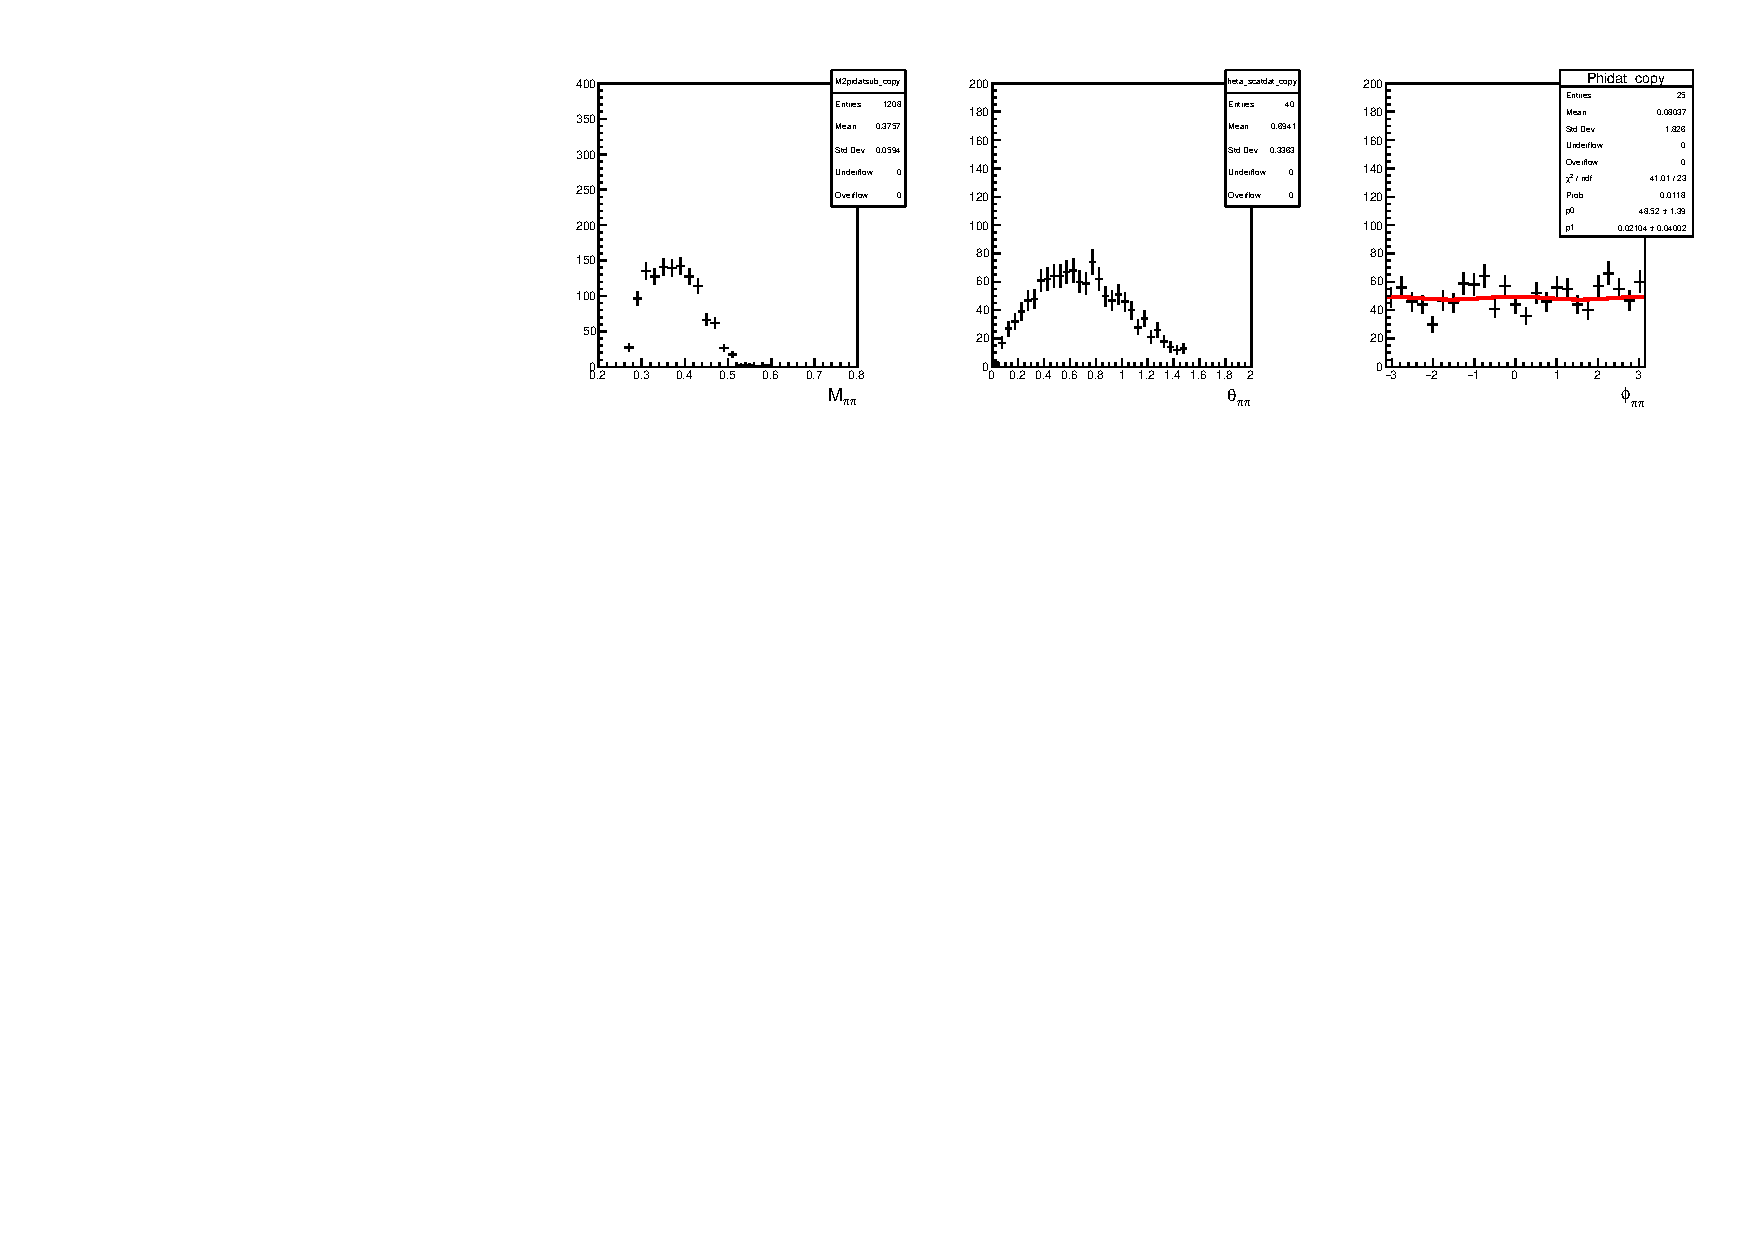
\includegraphics[width=16cm,clip=true]{figures/BrokenEtasPrim.pdf}
\caption{Kinematically fit distributions for broken $\eta$'s, that is $\eta$'s that decay to 3$\pi^0$, but get reconstructed with a reasonable probability as a 2$\pi^0$ final state.
We generated the sample using the {\em gen\_EtaPb} event generator using the Primakoff mechanism. The distributions produced from the NC mechanism are similar. 
Left) 2$\pi$ mass. Center) 2$\pi$ scattering angle. Right) 2$\pi$ azimuthal angle.
\label{fig:eta}}
\end{center} 
\end{figure}



\subsection{Miss-identified backgrounds}
There may be important backgrounds that are mistaken for the signal due to miss-identification. These may include
\begin{enumerate}[label=(\roman*)]
    \item coherent production of $\eta$ followed by $\eta\rightarrow \pi^0\pi^0\pi^0 \rightarrow \gamma\gamma\gamma\gamma(\gamma\gamma)$, where only four photons are reconstructed.
    \item production of nucleon resonances that contribute to the $\gamma N \rightarrow N \pi^0\pi^0$ final state. This contribution is expected to be small based on the experience of other Primakoff experiments.
\end{enumerate}
The most important background from miss-identification is due to $\eta$ production, where the $\eta$ decays to 3 pions but is reconstructed with a reasonable probability as a 2$\pi^0$ final state. We refer to these as ``broken" $\eta$'s. As with $\pi^0$ production, $\eta$ mesons may be produced via the Primakoff process, by the NC process or by quasi-elastic scattering from individual nucleons. The first two mechanisms are the most pernicious, as the incoherent production produces events that fall outside the typical signal kinematics. 
The incoherent production was investigated using the {\em genEtaRegge} event generator \cite{hdnote2437}. As expected, the resulting distributions are very similar to those from incoherent 2$\pi$ production described in the previous section.
If $\eta$'s are produced via the Primakoff and/or NC mechanisms, they may reconstruct as a 2$\pi$ final state if one of the decay pions is low energy and goes undetected. The probability for this to happen is at the percent level.  We describe these production mechanisms in more detail next.

Two samples of $\eta$ events were generated, one corresponding to Primakoff-$\eta$ production and the other due to NC production of $\eta$'s. These are two-body reactions, so they only differ in the angular distribution of the produced $\eta$, or equivalently their t-distribution. In principle these mechanisms interfere, but we generated the samples independent of one another and assuming a uniform azimuthal angular distribution. The events were then processed through the GEANT4 Monte Carlo, which decayed them according to their nominal branching fractions, and then {\em mcsmear}. These steps were followed by the reaction filter that analyzed the events just as if they were signal, i.e. treated events as $\gamma Pb \rightarrow Pb\, \pi^0 \pi^0$ with a kinematic fit assuming the recoil target nucleus was missing. 
%Standard missing-mass and $\chi^2$ cuts were used to pick out events that faked the signal. 
%It turns out that the angular distribution of broken $\eta$'s produced from the NC process are not very different than those for the Primakoff production shown in the figure.

We used a couple of very simple but powerful selection cuts to eliminate the $\eta$ background. The cuts include a selection on the missing mass squared ($|MM - M_{Pb}{^2}| < 0.1$ GeV$^2$) and a cut on the $\chi^2 < 5$ of the kinematic fit to $\gamma\,Pb\rightarrow \pi^0\pi^0 (Pb)$ with a missing recoil. In the analysis we also restrict the $2\pi$ scattering angle  ($\theta_{\pi\pi} <1.5$ degrees), which further constrains the range of missing mass. The result of these selections, which have been applied uniformly to signal and background, reduce the contamination from this source to about 37\% of the signal. The distributions of the accepted events for the Primakoff-$\eta$ mechanism are shown in Fig.\ref{fig:eta}. 
These selections are illustrative and will allow us to achieve our experimental goals but further optimizations are likely. We note that the relative number of miss-identified $\eta$'s in the experiment will be determined empirically from the measured rate of fully reconstructed $\eta\rightarrow\pi^0\pi^0\pi^0$ events.

The number of generated Primakoff-$\eta$ events was determined by using the scaling rules  described in Appendix\,\ref{sec:SigmaScaling}. The rate of Primakoff-$\eta$ production was determined relative to Primakoff-$\pi^0$ (0.28) and the results in the appendix (Eq.\,\ref{eq:sigpipi_over_sigpi}) used to determine this rate relative to Primakoff-$\pi^0\pi^0$ (1/0.05), resulting in $\sigma_\eta/\sigma_{\pi^0\pi^0} \sim 6$. We assume that the fraction of NC-$\eta$/Primakoff-$\eta \sim$ 1/3. The events from each sample were combined in this ratio as backgrounds for use in the study to the extraction of the signal.

 \begin{figure}[tbp]
\begin{center}
%\includegraphics[height=5cm,viewport=250 180 0 360,clip=true]{CPP_production3}
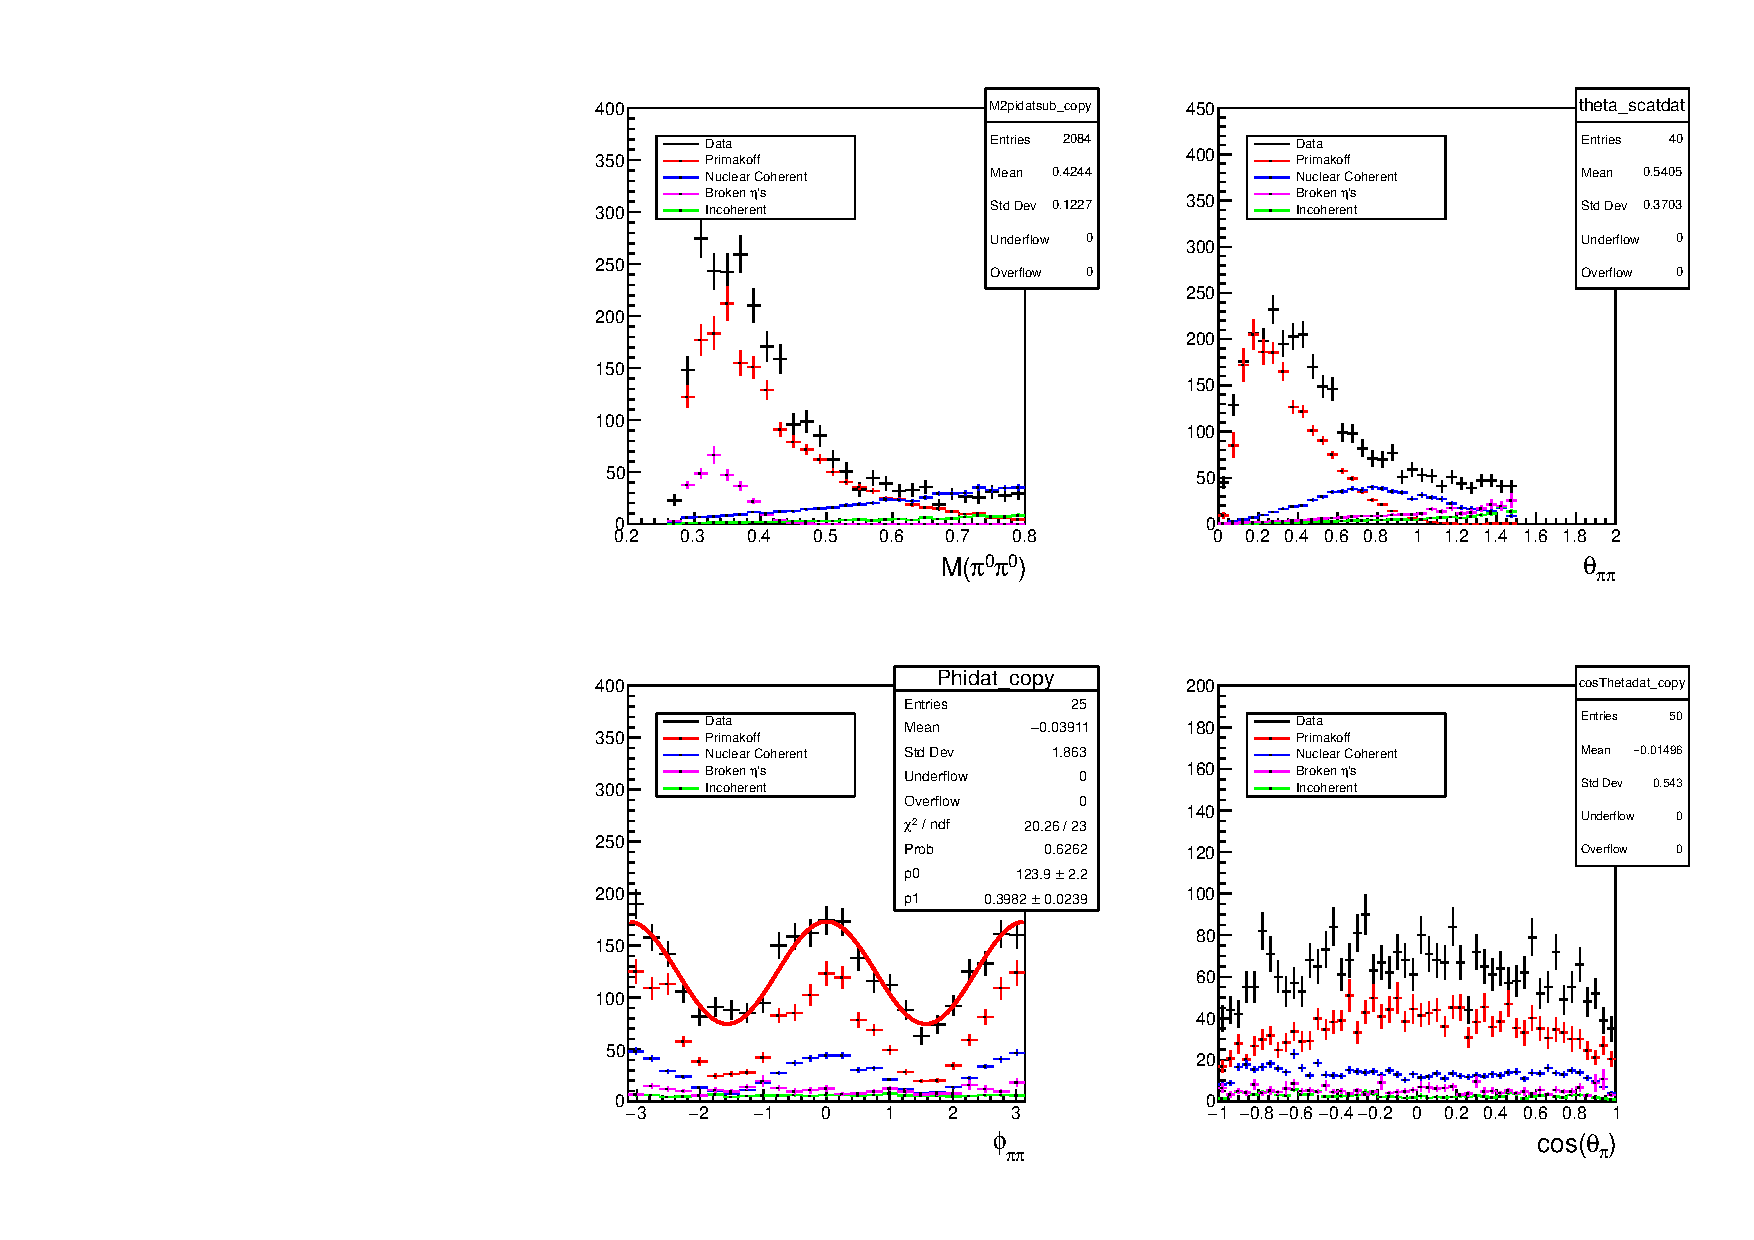
\includegraphics[height=15cm,clip=true]{figures/twopi_primakoff_DSelect_test_File_100000_decomposition_PrimNCICeta.pdf}
\caption{Results of the amplitude fit to the MC data (black points) to extract the amplitudes for the $\pi^0\pi^0$ Primakoff signal, nuclear coherent background, broken $\eta$ distributions and incoherent background.
Top left) 2$\pi$ mass, Top right) 2$\pi$ scattering angle, Bottom left) 2$\pi$ azimuthal angle, 
Bottom right) Polar angle of one pion in the $2\pi$ center-of-mass.
\label{fig:decomposition_PrimNCICeta}}
\end{center} 
\end{figure}

\subsection{Extraction of the Primakoff signal \label{sec:signalfit}}
The $\pi^0\pi^0$ Primakoff signal is determined using an amplitude fit\footnote{AmpTools, https://github.com/mashephe/AmpTools/wiki.} to all data simultaneously. It assumes that the mass and angular distributions are known for each of the contributions to the 2$\pi$ sample. A complex scaling factor is determined for each contribution by doing an unbinned maximum likelihood fit to the event sample. The result of such a fit to the sample that includes the Primakoff and NC processes only, is shown in  Fig.\,\ref{fig:decomposition_PrimNC}. The fit to the MC data that includes the Primakoff-$\pi^0\pi^0$ signal, and backgrounds from NC-$\pi^0\pi^0$, incoherent production and broken $\eta$'s, is shown in Fig.\,\ref{fig:decomposition_PrimNCICeta}. The generated samples correspond approximately to the expected number of events expected for the experiment. The three kinematic quantities that are most discriminating between the signal and background are the 2$\pi$ mass $M_{\pi\pi}$, the 2$\pi$ scattering angle $\theta_{\pi\pi}$ and the azimuthal angle $\phi_{\pi\pi}$. The fit uses all the kinematic information contained in the event sample to determine the fraction of signal and background components that are present. A good fit is obtained to the data and the Primakoff signal is determined. The statistical uncertainties as a function of $M_{\pi\pi}$ are obtained directly from the fit (Top left plot in Fig.\,\ref{fig:decomposition_PrimNCICeta}). We estimate the systematic uncertainty (3\%) in the extraction of the signal by
assuming that the number of broken $\eta$'s can be known with an uncertainty of 25\%.

